
%
%  $Description: Author guidelines and sample document in LaTeX 2.09$ 
%
%  $Author: John Burchell & William Granli $
%  $Date: 2015/01/21 15:20:59 $
%  $Revision: 1.0
%

\documentclass[10pt,twocolumn]{article} 
\usepackage{latex8}
\usepackage{url}
\usepackage{verbatim}
\usepackage{fixltx2e}
\usepackage{graphicx}
%\documentstyle[times,art10,twocolumn,latex8]{article}

%------------------------------------------------------------------------- 
% take the % away on next line to produce the final camera-ready version 
\pagestyle{empty}

%------------------------------------------------------------------------- 
\begin{document}



\title{Assignment 4}

% author names and affiliations
\author{John Burchell and William Granli \\
john.a.burchell, william.granli@gmail.com}


\maketitle
\thispagestyle{empty}

%------------------------------------------------------------------------- 


\Section{Methodology}
This section will describe which statistical tests were used, and why. The level of significance used for all tests is 0.05. 

\SubSection{Tests Used for H\textsubscript{eff} and H\textsubscript{rate}}
Initially, Kolmogorov-Smirnov (KS) Goodness-of-Fit and Shapiro-Wilks (SW) tests were used to determine if the assumption of normality could be held for the data set. The data used for the tests was the number faults found by each participant. The reason this data was chosen was that it directly correlates to the data used in H\textsubscript{eff} and H\textsubscript{rate}. The KS and SW tests both reported p-values < 0.05. See Table 1 for the p-values of the KS and SW tests. The critical value analysis for the KS and SW showed similar results and thus the null hypotheses of the data being normally distributed was rejected. See Table 2 for more information about the critical value results of the KS and SW tests.

\begin{table}
	\centering
	\begin{tabular}[Ht]{| l | l | l |}
	\hline
	Test & Sample & p-value  \\
	\hline
	KS & UC & \textless 2.2e-16 \\
	\hline
	SW & UC & 0.000969 \\
	\hline
	KS & CL & \textless 2.2e-16 \\
	\hline
	SW & CL & 0.309 \\	
	\hline
	\end{tabular}
	\caption{KS \& SW tests - p-value}
\end{table}


\begin{table}
	\centering
	\begin{tabular}[Ht]{| l | l | l | l |}
	\hline
	Test & Sample & Critical Value & D (result)  \\
	\hline
	KS & UC & 0.270 & 0.9388 \\
	\hline
	SW & UC & 0.964 &  0.8412 \\
	\hline
	KS & CL & 0.270 & 0.9388 \\
	\hline
	SW & CL & 0.964 & 0.9553 \\	
	\hline
	\end{tabular}
	\caption{KS \& SW tests - Critical Value}
\end{table}


A graphical representation of the level of normalisation can be seen in Figure 1 and 2. The results from the tests are supported by the sparseness of the data points. 

\begin{figure}[Ht]
\centering
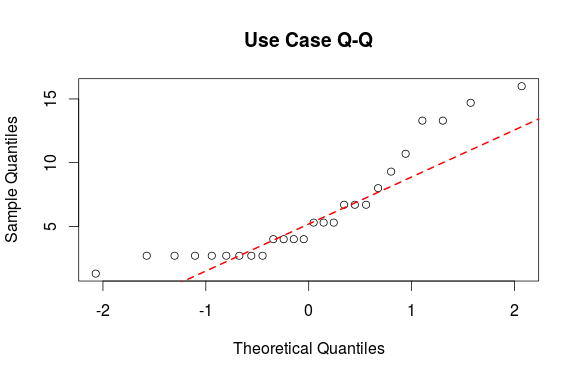
\includegraphics[width=90mm]{uc_qq.png}
\caption{Use Case Q-Q plot}
\end{figure}

\begin{figure}[Ht]
\centering
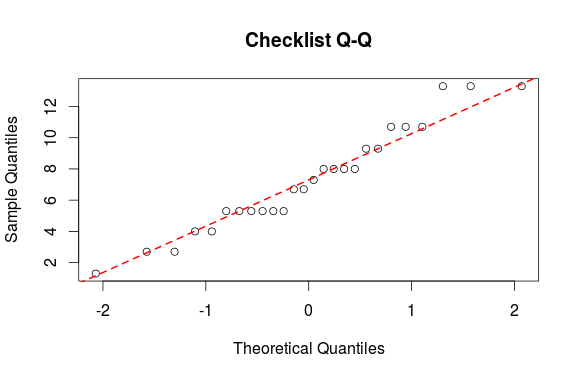
\includegraphics[width=90mm]{cl_qq.png}
\caption{Checklist Q-Q plot}
\end{figure}


The next step was to perform an outlier test. The method used was boxplots. As seen in Figure 3 and 4, no outliers were detected and thus no data points were removed in the tests performed. 

\begin{figure}[Ht]
\centering
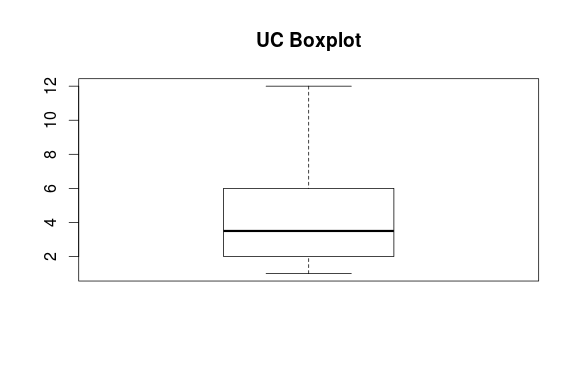
\includegraphics[width=90mm]{uc_box.png}
\caption{Use Case Boxplot}
\end{figure}

\begin{figure}[Ht]
\centering
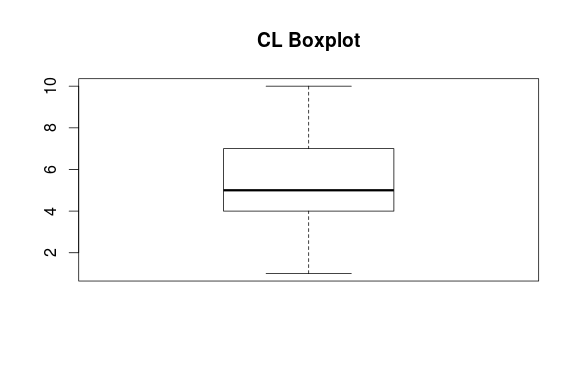
\includegraphics[width=90mm]{cl_box.png}
\caption{Checklist Boxplot}
\end{figure}


\Section{Results}

\subsection{first hypothesis}
Since the data is non-normalised, the Wilcoxon-Mann-Whitney (WMW) two-sample rank-sum teset was chosen instead of the Student's T-test as the final test. The data used for the WMW test was the efficiency of each participant. The result of the WMW test was W=250, p=0.1063 and with the significance level of 536 H0 is rejected. 

\subsection{second hyphothesis}


http://www.sussex.ac.uk/Users/grahamh/RM1web/WilcoxonTable2005.pdf



MWW = good for cont tests as well.
 Mann, Henry B.; Whitney, Donald R. (1947). "On a Test of Whether one of Two Random Variables is Stochastically Larger than the Other". Annals of Mathematical Statistics 18 (1): 50–60. doi:10.1214/aoms/1177730491. MR 22058. Zbl 0041.26103.







\Section{Tests for eff}


\Section{Tests for 3}



Chi-square test requirements[edit]
Quantitative data.
One or more categories.
Independent observations.
Adequate sample size (at least 10).
Simple random sample.
Data in frequency form.
All observations must be used.
\bibliographystyle{latex8}
\bibliography{latex8}


\Section{Acknowledgements}
U w0T m8


\end{document}

